% ORIGIN: A Real-Time Multi-Messenger Superevent Manager
% for Gravitational-Wave Follow-Up
% Prepared for submission to ApJ

\documentclass[twocolumn]{article}

\usepackage{amsmath}
\usepackage{amssymb}
\usepackage{listings}
\usepackage{booktabs}
\usepackage{url}
\usepackage{graphicx}
\usepackage[margin=1in]{geometry}
\usepackage{natbib}
\usepackage[pdfencoding=auto,psdextra]{hyperref}

% AAS journal macros
\let\apj\undefined\let\apjl\undefined\let\mnras\undefined\let\pasp\undefined\let\aap\undefined
\newcommand{\apj}{ApJ}
\newcommand{\apjl}{ApJL}
\newcommand{\mnras}{MNRAS}
\newcommand{\pasp}{PASP}
\newcommand{\aap}{A\&A}
\newcommand{\arcdeg}{\ensuremath{{}^{\circ}}}

\lstset{
  basicstyle=\ttfamily\small,
  frame=single,
  breaklines=true,
  columns=fullflexible,
}

\begin{document}

\title{ORIGIN: A Real-Time Multi-Messenger Superevent Manager for Gravitational-Wave Follow-Up}

\author{Michael W. Coughlin}
\date{}

\maketitle

\begin{abstract}
We present ORIGIN (\textbf{O}bservatory for \textbf{R}eal-time \textbf{I}nference of \textbf{G}ravitational and Electromagnetic \textbf{N}etworks), a modular, high-performance framework for real-time correlation of gravitational-wave (GW) events with electromagnetic (EM) and neutrino counterparts. Written in Rust and designed for the LIGO--Virgo--KAGRA O4/O5 observing runs, ORIGIN ingests alerts from NASA's General Coordinates Network (GCN), the Zwicky Transient Facility (ZTF) via the BOOM broker, and simulated event streams. The system implements a RAVEN-compatible joint false-alarm rate (FAR) statistic combining temporal coincidence, HEALPix skymap spatial integration, and light-curve-based source classification to identify significant multi-messenger superevents. We calibrate the full pipeline on an O4 observing scenario population of 178 BNS/NSBH events with $1{,}000$ background trials each, characterizing spatial discrimination for Fermi-GBM (${\sim}9\times10^{4}\times$ median signal-to-background ratio), Swift-BAT, and optical counterparts. Temporal discrimination via SVI-based $t_0$ recovery provides an additional ${\sim}17\times$ rejection factor, while early linear rate classification correctly penalizes $>97\%$ of supernova contaminants with zero false boosting. An end-to-end analysis combining all stages yields a cumulative background rejection of ${\sim}200\times$ when SVI $t_0$ fitting succeeds, reducing ${\sim}1{,}000$ ZTF candidates to ${\sim}5$ expected false associations per GW event, or ${\sim}79\times$ when falling back to per-measurement temporal matching (${\sim}13$ false associations). ORIGIN processes GRB correlations at sub-second latency and is publicly available at \url{https://github.com/mcoughlin/origin}.
\end{abstract}

\paragraph{Keywords:} gravitational waves --- methods: data analysis --- gamma-ray burst: general --- surveys --- stars: neutron

\section{Introduction} \label{sec:intro}

The binary neutron star merger GW170817 \citep{Abbott2017a, Abbott2017b} and its electromagnetic counterparts---the short gamma-ray burst GRB~170817A \citep{Goldstein2017, Abbott2017c}, the kilonova AT~2017gfo \citep{Coulter2017, Kasen2017, Villar2017}, and a multi-wavelength afterglow---inaugurated the era of multi-messenger astronomy with gravitational waves. This single event demonstrated the transformative potential of combining information across messenger channels, yielding constraints on the neutron-star equation of state \citep{Dietrich2020}, an independent measurement of the Hubble constant, and direct evidence for $r$-process nucleosynthesis in merging neutron stars \citep{Lattimer1974, Siegel2019, Levan2024}.

As the LIGO--Virgo--KAGRA (LVK) detector network progresses through its fourth (O4) and into its fifth (O5) observing run, the rate of detectable compact binary coalescence events continues to grow \citep{Abbott2020, GWTC4, GWTC4pop}, with several BNS mergers expected per year at O5 sensitivity. The LVK low-latency alert infrastructure now routinely issues public alerts within seconds of detection \citep{Chaudhary2024, LVK2019lowlatency}. Simultaneously, wide-field optical surveys such as the Zwicky Transient Facility \citep[ZTF;][]{Bellm2019, Graham2019}, ATLAS \citep{Tonry2018}, and GOTO \citep{Steeghs2022} detect thousands of transients per night, and the upcoming Vera C.\ Rubin Observatory Legacy Survey of Space and Time \citep[LSST;][]{Ivezic2019} will increase this volume by an order of magnitude. In the gamma-ray domain, \textit{SVOM} \citep{Wei2016} now provides ${\sim}60$ GRBs per year, complementing the aging but still operational \textit{Fermi} and \textit{Swift} missions. \textit{Einstein Probe} \citep{EinsteinProbe2025} adds X-ray transient detections at a rate of roughly one per ten days. Together, these facilities create a rich but fragmented multi-messenger landscape in which rare astrophysical associations must be identified against a large combinatorial background of unrelated events.

A layered ecosystem of tools has emerged to address this challenge. Alert brokers such as AMPEL \citep{Nordin2019}, Fink \citep{Moller2021}, and BOOM (Coughlin et al., in prep.) filter and classify high-rate optical alert streams. Science platforms like SkyPortal \citep{Coughlin2023} and Treasure Map \citep{Wyatt2020} aggregate and contextualize multi-facility observations. Telescope coordination networks including GRANDMA \citep{Antier2020}, GROWTH \citep{Coughlin2019a}, and GECKO \citep{Kim2022} organize follow-up campaigns. On the GW+GRB side, RAVEN \citep{Urban2016} performs real-time temporal-spatial coincidence searches within the LVK low-latency pipeline. Bayesian inference frameworks such as NMMA \citep{Pang2023} enable joint analysis of multi-messenger data. Machine-learning approaches to counterpart identification are also maturing \citep{Sravan2024}.

Despite these advances, no existing public system provides an integrated, real-time correlation engine that simultaneously ingests alerts from multiple Kafka brokers with heterogeneous authentication, performs HEALPix-based spatial correlation using full GW probability skymaps, applies light-curve-based source classification to discriminate kilonovae from background supernovae, and computes a unified joint FAR statistic across all messenger channels. Multi-messenger follow-up remains largely structured around isolated alerts from individual discovery streams, without a unified framework that associates heterogeneous signals with a single, evolving astrophysical origin in real time.

In this paper, we present ORIGIN, a Rust-based multi-messenger superevent manager that fills this gap. ORIGIN adopts a physically motivated \textit{superevent} paradigm in which alerts from gravitational-wave detectors, gamma-ray satellites, X-ray telescopes, and optical surveys are continuously associated with a common astrophysical origin and updated as new observations become available. Section~\ref{sec:architecture} describes the system architecture. Section~\ref{sec:correlation} details the correlation algorithms. Section~\ref{sec:lightcurve} presents the light curve analysis pipeline. Section~\ref{sec:calibration} presents the FAR calibration on an O4 observing scenario population. Section~\ref{sec:discussion} discusses performance, comparison with existing systems, and future directions.

\section{System Architecture} \label{sec:architecture}

\subsection{Design Principles} \label{sec:design}

ORIGIN is implemented in Rust for memory safety, zero-cost abstractions, and high-throughput concurrent I/O via the Tokio async runtime. The system is organized as a workspace of nine specialized crates following a layered architecture. Table~\ref{tab:crates} summarizes the role of each crate.

% TODO: Add architecture figure
% \begin{figure}
% \plotone{figures/architecture.pdf}
% \caption{ORIGIN system architecture.\label{fig:architecture}}
% \end{figure}

\begin{table*}[htbp]
\centering
\caption{ORIGIN workspace crates and their responsibilities. \label{tab:crates}}
\begin{tabular}{ll}
\toprule
Crate & Description \\
\midrule
\texttt{mm-core}       & Foundational types, fitting algorithms, and feature extraction \\
\texttt{mm-correlator} & Correlation engine with temporal indices and superevents \\
\texttt{mm-gcn}        & GCN Kafka consumer (OAUTHBEARER); GW/GRB/neutrino parsers \\
\texttt{mm-boom}       & BOOM/ZTF Kafka consumer (SCRAM-SHA-512); Avro deserialization \\
\texttt{mm-simulation} & Background generation, GRB simulation, and injection testing \\
\texttt{mm-config}     & TOML-based configuration with environment variable overrides \\
\texttt{mm-redis}      & State persistence via Redis for fault tolerance \\
\texttt{mm-api}        & REST API (Actix-web) for external consumers \\
\texttt{mm-service}    & CLI binaries for streaming, correlation, and analysis \\
\bottomrule
\end{tabular}
\end{table*}

At the foundation, \texttt{mm-core} defines the shared domain types and algorithms used throughout the system. The \texttt{mm-correlator} crate builds on these types to implement the temporal indexing and superevent aggregation logic described in Section~\ref{sec:correlation}. Two data ingestion crates, \texttt{mm-gcn} and \texttt{mm-boom}, handle the protocol-specific details of consuming from NASA's GCN and Caltech's BOOM Kafka brokers, respectively. The \texttt{mm-simulation} crate provides synthetic event generation for testing and validation. Supporting infrastructure is provided by \texttt{mm-config} (configuration), \texttt{mm-redis} (persistence), and \texttt{mm-api} (external access), while \texttt{mm-service} packages the system into deployable CLI binaries.

\subsection{Data Ingestion} \label{sec:ingestion}

ORIGIN consumes alerts from two real-time Kafka streams. The first is the General Coordinates Network (\texttt{kafka.gcn.nasa.gov}), which distributes alerts from all major time-domain instruments. ORIGIN subscribes to LVK gravitational-wave alerts \citep{Chaudhary2024, LVK2019lowlatency} on the \texttt{igwn.gwalert} topic (JSON with skymap URLs), Fermi-GBM GRB positions via the \texttt{gcn.classic.voevent.FERMI\_GBM\_*} topics (VOEvent XML), Swift-BAT GRBs on \texttt{gcn.notices.swift.bat.guano} (Avro), \textit{Einstein Probe} \citep{EinsteinProbe2025} X-ray transients on \texttt{gcn.notices.einstein\_probe.wxt.alert}, and IceCube high-energy neutrino tracks on \texttt{gcn.notices.icecube.*}. Authentication uses OAUTHBEARER with a custom token-refresh callback that fetches tokens from \texttt{auth.gcn.nasa.gov}, bypassing librdkafka's built-in OIDC implementation which is unreliable on some platforms.

The second stream is the BOOM broker (\texttt{kaboom.caltech.edu:9093}; Coughlin et al., in prep.), which delivers classified ZTF transient alerts. ORIGIN subscribes to nine \texttt{babamul.ztf.*} topics covering stellar, hosted, and hostless transients across multiple partnership tiers. Authentication uses SASL/SCRAM-SHA-512. Alerts are Apache Avro-encoded with a nested \texttt{candidate} sub-record containing photometry (\texttt{ra}, \texttt{dec}, \texttt{jd}, \texttt{magpsf}, \texttt{sigmapsf}, \texttt{band}) and a \texttt{prv\_candidates} array of historical detections.

\subsection{Superevent Data Model} \label{sec:datamodel}

The central data structure is the \texttt{MultiMessengerSuperevent}, which aggregates coincident events across all messenger channels:

\begin{lstlisting}
MultiMessengerSuperevent {
    id: String,
    t_0: f64,
    gw_event: Option<GWComponent>,
    optical_candidates:
        Vec<OpticalCandidate>,
    gamma_ray_candidates:
        Vec<GammaRayCandidate>,
    xray_candidates:
        Vec<XRayCandidate>,
    neutrino_candidates:
        Vec<NeutrinoCandidate>,
    joint_far: Option<f64>,
}
\end{lstlisting}

Each \texttt{GWComponent} stores the superevent ID, GPS time, instrument list, FAR, sky position, and (when available) a parsed HEALPix skymap. Each \texttt{OpticalCandidate} stores the object ID, detection time, sky position, time offset from the GW trigger, spatial offset, joint FAR, and light curve features including early rates and GP-derived parameters.

\section{Correlation Algorithms} \label{sec:correlation}

\subsection{Temporal Matching} \label{sec:temporal}

ORIGIN maintains a \texttt{TemporalIndex} backed by a \texttt{BTreeMap} providing $\mathcal{O}(\log n)$ insertion and range queries. When a new event arrives, the index is queried for all superevents within a configurable time window. For GRB searches, the default window is $[-1, +60]$~seconds relative to the GW trigger, following RAVEN conventions for short GRBs. For optical counterpart searches, the window is extended to $[-1, +86400]$~seconds, since the optical counterpart of a BNS merger may not be detected until hours after the GW trigger due to survey cadence constraints. For historical replay, ORIGIN uses a fresh Kafka consumer group per run with \texttt{auto.offset.reset=earliest} to replay all available data from the beginning.

\subsection{Spatial Correlation via HEALPix Skymap Integration} \label{sec:spatial}

When a GW event includes a HEALPix probability skymap (typically at $\mathrm{NSIDE} = 512$, giving $12 \times 512^2 \approx 3.1$ million pixels and ${\sim}0.013~\mathrm{deg}^2$ per pixel), ORIGIN performs spatial correlation by integrating the skymap probability over the counterpart's position uncertainty region.

For gamma-ray bursts with large error circles (typically 1--15~degrees for Fermi-GBM), the integration uses the BMOC (Basic Multi-Order Coverage) cone approximation from the \texttt{cdshealpix} library:
\begin{equation} \label{eq:pspatial}
    P_\mathrm{spatial} = \sum_{i \in \mathrm{cone}(r)} p_i
\end{equation}
where $p_i$ is the probability in HEALPix pixel $i$ and the cone radius $r$ is the GRB error radius. For well-localized sources (error $< 0.1$~degrees, e.g., ZTF transients with ${\sim}2$~arcsecond positions), the probability is queried at a single pixel.

ORIGIN also computes credible region membership: whether the counterpart position falls within the 50\% or 90\% credible region of the GW skymap, and a spatial significance score normalized against the maximum-probability pixel.

\subsection{Joint False Alarm Rate} \label{sec:far}

Following the RAVEN framework \citep{Urban2016}, the expected number of false coincidences per GW event is:
\begin{equation} \label{eq:farjoint}
    N_\mathrm{false} = R_\mathrm{ext} \cdot \Delta T \cdot P_\mathrm{spatial} \cdot N_\mathrm{trials}
\end{equation}
where $R_\mathrm{ext}$ is the external event rate (e.g., 325~GRBs/year for the combined Fermi-GBM + Swift-BAT + SVOM-ECLAIRs sample), $\Delta T$ is the temporal coincidence window, $P_\mathrm{spatial}$ is the skymap overlap probability, and $N_\mathrm{trials}$ accounts for the number of independent search bands (default: 7 for the ZTF filter set and GRB energy bands).

For the full RAVEN spatiotemporal FAR:
\begin{equation} \label{eq:farraven}
    \mathrm{FAR}_\mathrm{RAVEN} = \frac{\Delta T \cdot R_\mathrm{ext} \cdot \mathrm{FAR}_\mathrm{GW}}{P_\mathrm{spatial}}
\end{equation}

A coincidence is considered significant when $\mathrm{FAR}_\mathrm{joint}$ falls below a threshold of 1/30~per~year (approximately one false alarm per month), configurable via the \texttt{far\_threshold} parameter.

\subsection{Light-Curve-Based FAR Adjustment} \label{sec:lcfar}

The joint FAR is further modulated by light curve properties to discriminate kilonovae (KN) from background supernovae (SN):
\begin{equation} \label{eq:faradj}
    \mathrm{FAR}_\mathrm{adjusted} = \mathrm{FAR}_\mathrm{joint} \times f_\mathrm{early} \times f_\mathrm{GP}
\end{equation}
where $f_\mathrm{early}$ is the early-rate multiplier (Section~\ref{sec:earlyrate}) and $f_\mathrm{GP}$ is the Gaussian Process feature penalty (Section~\ref{sec:gp}). A KN-like light curve ($f < 1$) boosts significance, while a SN-like curve ($f > 1$) suppresses it.

\section{Light Curve Analysis Pipeline} \label{sec:lightcurve}

\subsection{Early Linear Rate Discriminator} \label{sec:earlyrate}

Kilonovae evolve on timescales of hours to days \citep{Metzger2017, Kasen2017}, significantly faster than Type~Ia supernovae which rise over ${\sim}15$~days \citep{Arnett1982}. ORIGIN exploits this difference through a fast, model-independent discriminator that requires as few as 2 detections. The algorithm groups photometric measurements by band, selects the best-sampled band, and identifies the epoch of peak brightness (minimum magnitude). A linear model is then fit to the pre-peak (rising) measurements via ordinary least squares to obtain the rise rate $\dot{m}_\mathrm{rise}$ (mag/day), and separately to the post-peak (fading) measurements to obtain the decay rate $\dot{m}_\mathrm{decay}$ (mag/day).

The resulting rates are mapped to FAR multipliers according to the thresholds in Table~\ref{tab:earlyrate}. Sources with fast photometric evolution characteristic of kilonovae receive a FAR boost (multiplier $< 1$), while slowly-evolving sources consistent with supernovae are penalized (multiplier $> 1$). Decay rates provide a secondary discriminant: kilonovae decay faster ($|\dot{m}_\mathrm{decay}| > 0.3$~mag/day) than most supernovae. Because the rise and decay multipliers are applied independently, the combined factor ranges from 0.09 (strong KN boost: $0.3 \times 0.3$) to 25.0 (strong SN penalty: $5.0 \times 5.0$).

\begin{table}[htbp]
\centering
\caption{Early rate discriminator classification thresholds and corresponding FAR multipliers. \label{tab:earlyrate}}
\begin{tabular}{lcc}
\toprule
Classification & Rise rate criterion & Multiplier \\
\midrule
KN-like      & $|\dot{m}_\mathrm{rise}| > 1.0$~mag/day & 0.3 (boost) \\
Intermediate & $0.5 \leq |\dot{m}_\mathrm{rise}| \leq 1.0$~mag/day & 1.0 (neutral) \\
SN-like      & $|\dot{m}_\mathrm{rise}| < 0.5$~mag/day & 5.0 (penalize) \\
\bottomrule
\end{tabular}
\end{table}

This discriminator is designed to operate on the sparse, early light curves typical of ZTF cadence (1--3 day revisit), where sophisticated model fitting may not yet be possible.

\subsection{Gaussian Process Feature Extraction} \label{sec:gp}

For light curves with 3 or more detections, ORIGIN extracts morphological features via Gaussian Process (GP) regression. The GP uses a composite kernel:
\begin{equation} \label{eq:gpkernel}
    K(t_i, t_j) = A \cdot \exp\!\left(-\frac{(t_i - t_j)^2}{2\ell^2}\right) + \sigma_n^2 \delta_{ij}
\end{equation}
where $A$ is the amplitude, $\ell$ is the lengthscale, and $\sigma_n^2$ is the noise variance. Hyperparameters are selected via grid search over amplitudes $A \in \{0.05, 0.1, 0.2, 0.4\}$ and lengthscale factors $\ell/T \in \{1, 2, 4, 8, 16\}$ (where $T$ is the light curve duration), minimizing the negative log marginal likelihood.

From the GP posterior prediction (evaluated at 50 uniformly spaced points), the system extracts the rise rate (linear regression slope over the first 25\% of predictions), the decay rate (slope over the last 25\%), the peak magnitude (minimum GP prediction), the FWHM (duration in days at half the peak flux above baseline), and flux derivatives $df/dt$ at all prediction points (capturing the maximum, minimum, and current rates of change). These features are combined into a background rejection score that multiplies the joint FAR.

\subsection{Explosion Time Estimation} \label{sec:t0}

Accurate estimation of the explosion/merger time $t_0$ is critical for temporal correlation with GW events. ORIGIN implements two complementary approaches.

The first is simple linear extrapolation: a linear model is fit to the rising portion of the light curve (flux vs.\ time) and solved for flux~$= 0$, giving $t_0 = -b/m$ where $m$ is the slope and $b$ the intercept. Sanity checks ensure $t_0$ precedes the first detection by no more than 30~days.

The second approach uses Stochastic Variational Inference (SVI) to fit the light curve to a physical kilonova model \citep{Metzger2010}, parameterized by ejecta mass $M_\mathrm{ej}$, ejecta velocity $v_\mathrm{ej}$, opacity $\kappa$, and explosion time $t_0$. The fitting procedure consists of three stages. First, Particle Swarm Optimization (PSO) with 40 particles explores the parameter space for 100--200 iterations to identify a good starting point; for the Bazin model, a preliminary grid search over $(t_0, \tau_\mathrm{rise}, \tau_\mathrm{fall})$ with analytically-solved amplitude constrains the PSO search bounds and breaks the strong $t_0$--timescale degeneracies. Second, SVI refinement optimizes a mean-field Gaussian variational distribution $q(\theta) = \prod_i \mathcal{N}(\mu_i, \sigma_i^2)$ via the reparameterization trick \citep{Kingma2014} using Adam \citep{Kingma2015} for 1,000--5,000 iterations, with the ELBO (Evidence Lower Bound) as the optimization objective. The variational standard deviations are inflated by a factor of $4\times$ post-optimization to correct for the systematic underestimation of posterior variance inherent to mean-field approximations (calibrated via P-P plots on synthetic light curves following the ZTF lightcurve-fitting pipeline). Third, for empirical models (Bazin, Villar, PowerLaw), a cheap profile-likelihood sweep refines the $t_0$ estimate: the fitted $t_0$ is swept on a 50-point grid while holding other parameters at their SVI posterior means, analytically re-fitting the amplitude via weighted least squares at each point. The profile peak gives a bias-corrected $t_0$ and the profile curvature (via parabolic interpolation) gives a calibrated $1\sigma$ uncertainty. This refinement costs ${\sim}50$ model evaluations---negligible compared to the ${\sim}80{,}000$ evaluations of the SVI stage.

Four model families are available: Bazin \citep[empirical SN;][]{Bazin2009}, Villar \citep[improved empirical;][]{Villar2019}, PowerLaw (general transient), and MetzgerKN \citep[physical kilonova;][]{Metzger2010}. Upper limits are handled via a censored Gaussian likelihood:
\begin{equation} \label{eq:censored}
    \log p(f_\mathrm{lim} \mid f_\mathrm{pred}) = \log \Phi\!\left(\frac{f_\mathrm{lim} - f_\mathrm{pred}}{\sigma}\right)
\end{equation}
where $\Phi$ is the standard normal CDF.


\section{O4 Observing Scenario Calibration} \label{sec:calibration}

We calibrate ORIGIN's correlation pipeline using an O4 observing scenario injection set consisting of 178 simulated BNS and NSBH merger events with realistic HEALPix skymaps drawn from the LVK population. For each GW event, we generate 1,000 background trials by drawing random sky positions from a uniform distribution and computing the spatial probability against the GW skymap, yielding a total of 178,000 background simulations. Signal trials place the EM counterpart at the true merger location, offset within the instrument-specific error circle to simulate realistic detector localization uncertainty. This procedure is repeated independently for Fermi-GBM, Swift-BAT, and optical (ZTF/LSST) counterpart searches.

\subsection{GRB Spatial Discrimination} \label{sec:grb_spatial}

Figure~\ref{fig:grb_far} shows the spatial probability distributions for signal (true GRB counterpart at the merger location) and background (random sky position) trials for both Fermi-GBM and Swift-BAT. Table~\ref{tab:grb_calibration} summarizes the key metrics.

\begin{figure*}[htbp]
    \centering
    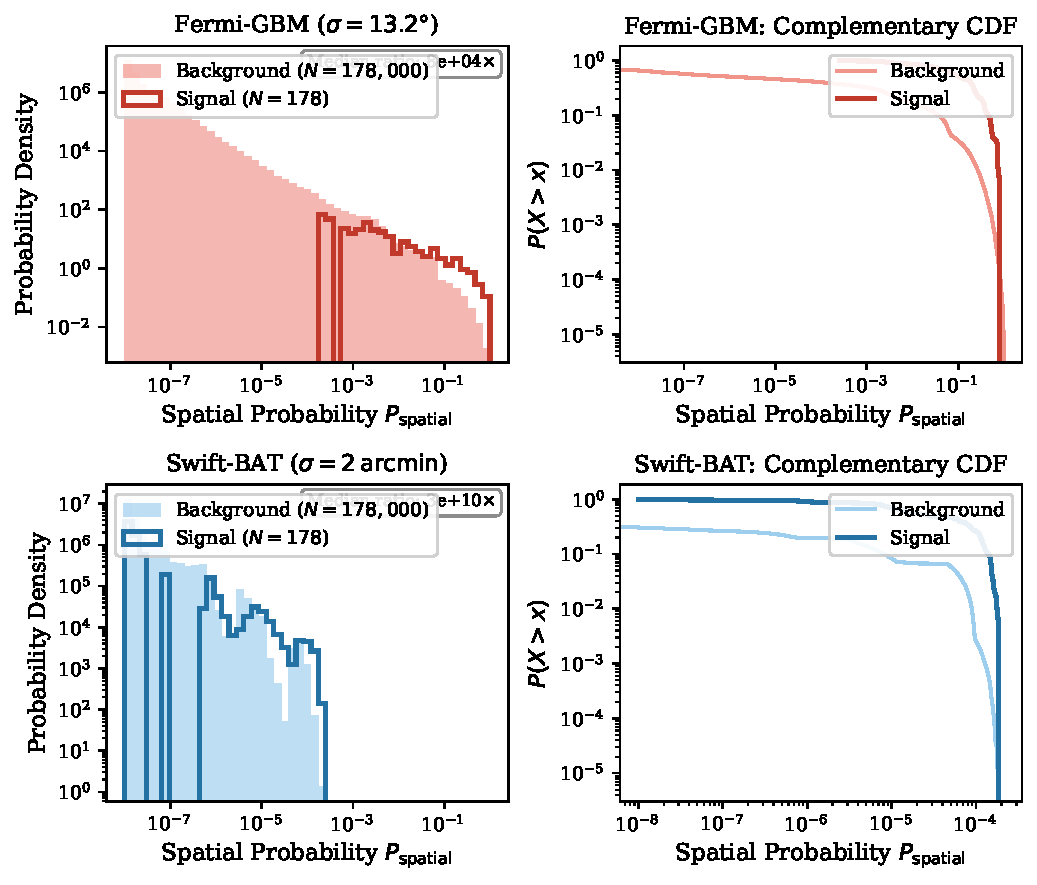
\includegraphics[width=\textwidth]{figures/far_calibration_grb.pdf}
    \caption{Spatial probability distributions for GRB counterpart searches in the O4 population. \emph{Top row}: Fermi-GBM with empirically-derived error radius of $13.2\arcdeg$ (median of 5,832 real detections). \emph{Bottom row}: Swift-BAT with $2$~arcmin error radius. Left panels show probability density histograms; right panels show complementary CDFs. In both cases, signal distributions (step lines) are clearly separated from background (filled histograms). \label{fig:grb_far}}
\end{figure*}

\begin{table*}[htbp]
\centering
\caption{Spatial probability calibration results for the O4 population (178 events $\times$ 1,000 background trials). Signal trials place the counterpart at the true merger location with a random offset within the instrument error circle. \label{tab:grb_calibration}}
\begin{tabular}{lcccc}
\toprule
Metric & Fermi-GBM & Swift-BAT & Optical (KN) & Optical (SN bg) \\
\midrule
Error radius                        & $13.2\arcdeg$   & $2\,\mathrm{arcmin}$  & $2\,\mathrm{arcsec}$ & $2\,\mathrm{arcsec}$ \\
Median $P_\mathrm{spatial}$ (signal)    & $1.18 \times 10^{-1}$    & $2.66 \times 10^{-5}$  & $2.86 \times 10^{-5}$ & --- \\
Median $P_\mathrm{spatial}$ (background) & $1.3 \times 10^{-6}$   & $0$ & $0$ & $0$ \\
Median discrimination ratio         & $9.1 \times 10^{4}$ & $\infty^{\dagger}$ & $\infty^{\dagger}$ & --- \\
Mean signal / mean background       & $12.8\times$     & $10.1\times$          & $10.2\times$          & --- \\
Signal zero-prob.\ fraction    & $0.0\%$          & $0.0\%$               & $0.0\%$               & --- \\
Background zero-prob.\ fraction & $32.4\%$        & $68.0\%$              & $68.1\%$              & --- \\
\bottomrule
\multicolumn{5}{l}{\footnotesize $^\dagger$ Background median is zero; median ratio is formally infinite.} \\
\end{tabular}
\end{table*}

For Fermi-GBM, we adopt an error radius of $13.2\arcdeg$, derived empirically from analysis of 5,832 real Fermi-GBM detections in the VOEvent archive. This value is $2.6\times$ larger than the commonly cited ${\sim}5\arcdeg$ and significantly affects spatial FAR calculations. Despite this large error circle, the median signal probability of $P_\mathrm{spatial} = 0.118$ is separated from the background median of $1.3\times10^{-6}$ by a factor of ${\sim}9\times10^4$, demonstrating strong spatial discrimination. All 178 signal trials yield nonzero spatial probability, while 32.4\% of background trials return zero. The mean signal-to-background ratio is $12.8\times$, lower than the median ratio because the median is dominated by the large fraction of background trials with negligible probability; both metrics are relevant depending on whether one is interested in typical or worst-case discrimination.

Swift-BAT achieves even stronger discrimination. Its tight 2~arcmin error circle yields lower absolute spatial probabilities (median signal $P_\mathrm{spatial} = 2.66\times10^{-5}$), but the background median drops to exactly zero, with 68.0\% of background trials having zero overlap with the GW skymap. The mean signal-to-background ratio of $10.1\times$ is comparable to Fermi-GBM, but the formally infinite median ratio (signal/zero) reflects the fact that most random sky positions have zero probability under the GW skymap at this angular resolution. Notably, Swift-BAT's 2~arcmin error circle and the 2~arcsecond optical position error both fall below the HEALPix pixel scale at $\mathrm{NSIDE}=512$ (${\sim}6.9$~arcmin), so both reduce to single-pixel queries and yield very similar spatial probability distributions.

\subsection{Optical Spatial Discrimination} \label{sec:optical_spatial}

The optical counterpart search uses the same O4 population with 2~arcsecond position errors characteristic of ZTF and LSST astrometry. Figure~\ref{fig:optical_far} compares the spatial probability distributions for simulated kilonova signals (placed at the merger location) against supernova background (random positions within the search area).

\begin{figure*}[htbp]
    \centering
    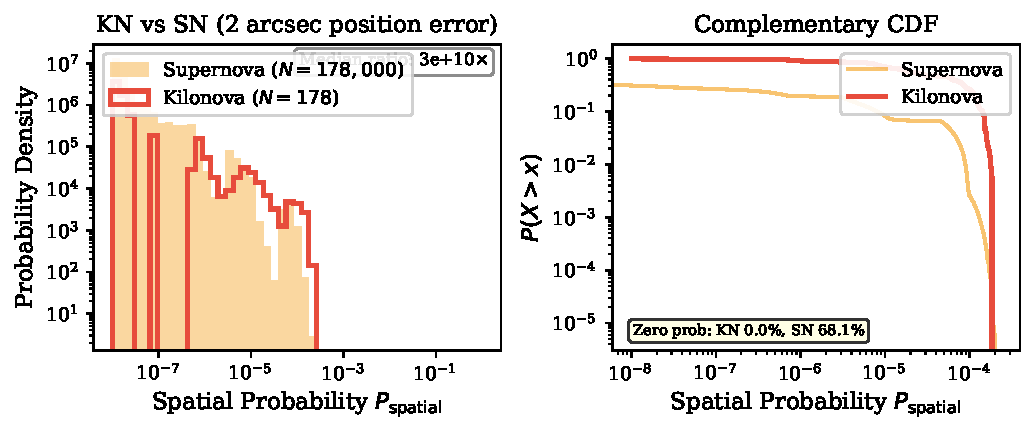
\includegraphics[width=\textwidth]{figures/far_calibration_optical.pdf}
    \caption{Spatial probability distributions for optical counterpart searches. Kilonova signals (step line) are placed at the true merger location; supernova background (filled histogram) is drawn from random positions. The 2~arcsecond optical position error resolves to a single HEALPix pixel at $\mathrm{NSIDE}=512$, yielding spatial probability distributions very similar to Swift-BAT (see text). \label{fig:optical_far}}
\end{figure*}

The optical channel yields a spatial probability distribution nearly identical to Swift-BAT, as expected from the single-pixel argument above: both instruments have error regions smaller than the HEALPix pixel size. The kilonova signal has zero zero-probability trials, while 68.1\% of supernova background trials have zero spatial overlap with the GW skymap. At higher skymap resolution ($\mathrm{NSIDE} = 2048$ or 4096, as sometimes used in LVK skymaps), Swift-BAT and optical would diverge, with the tighter optical localization providing stronger discrimination.

The key distinction between GRB and optical counterpart searches lies not in spatial discrimination but in temporal coincidence. GRBs arrive within seconds of the merger, providing extremely tight temporal constraints, whereas optical transients require a broader search window ($-1$~s to $+1$~day) due to survey cadence, making temporal discrimination more important for the optical channel.

\subsection{Temporal Discrimination via $t_0$ Recovery} \label{sec:t0_results}

To quantify the temporal discrimination power of the SVI $t_0$ fitter, we simulate 50 kilonova and 50 supernova light curves with realistic ZTF cadence (1--3 day revisit) and SNR~$=20$, fit each with its appropriate model (MetzgerKN for kilonovae, Bazin for supernovae), and compare the recovered $t_0$ against the true value. Figure~\ref{fig:t0} summarizes the results.

\begin{figure*}[htbp]
    \centering
    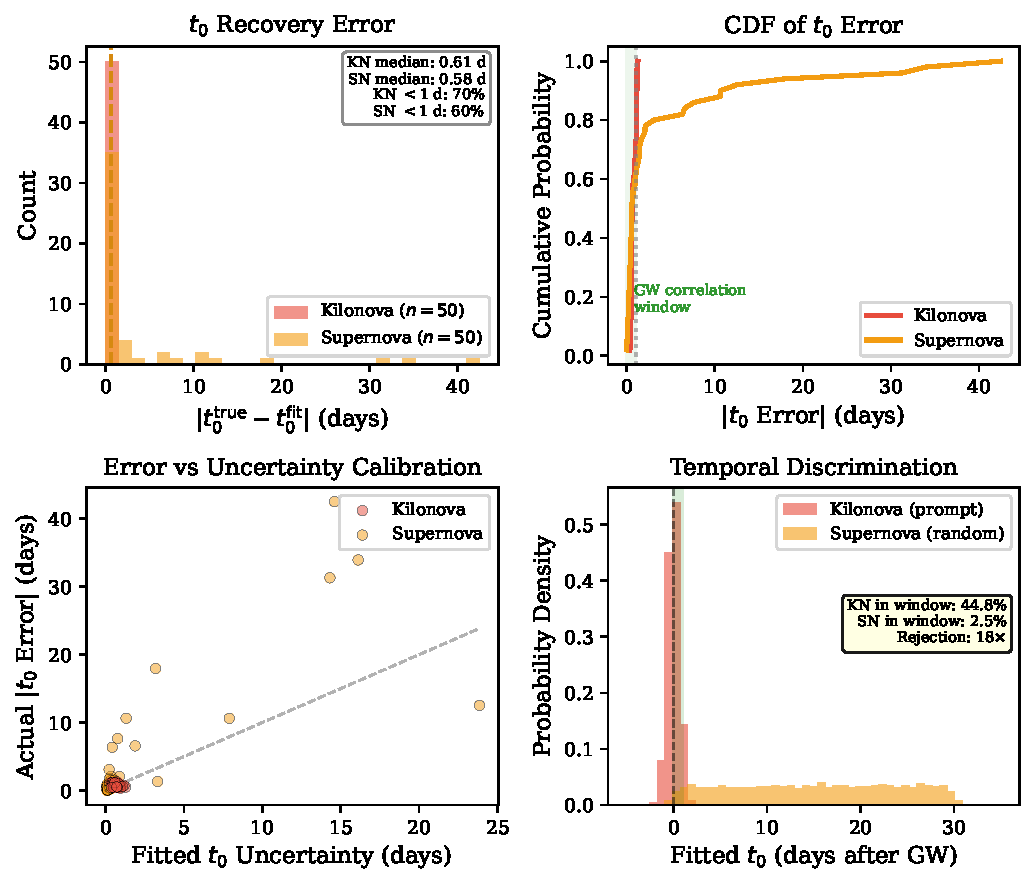
\includegraphics[width=\textwidth]{figures/t0_constraint_validation.pdf}
    \caption{Explosion time ($t_0$) recovery validation. \emph{Top left}: Distribution of $|t_0^\mathrm{true} - t_0^\mathrm{fit}|$ for kilonovae (red) and supernovae (orange), with median values indicated by dashed lines. \emph{Top right}: Cumulative distribution function; the green-shaded region marks the $\pm 1$~day GW correlation window. \emph{Bottom left}: Fitted $t_0$ uncertainty vs.\ actual error, showing that uncertainties are well-calibrated for kilonovae after $4\times$ sigma inflation (median uncertainty 0.73~days vs.\ median error 0.61~days). \emph{Bottom right}: Simulated temporal discrimination showing the distribution of fitted $t_0$ values relative to the GW merger time; kilonovae cluster near $t_0 = 0$ while supernovae are uniformly distributed. \label{fig:t0}}
\end{figure*}

Kilonovae are recovered with a median $t_0$ error of 0.61~days; 70\% of fitted $t_0$ values fall within 1~day of the true explosion time. The fitted $t_0$ uncertainty (median 0.73~days) is well-calibrated against the actual error thanks to the $4\times$ sigma inflation, validating the posterior calibration. Supernovae are recovered with a median $t_0$ error of 0.58~days for the well-constrained majority, though a long tail of poorly-constrained fits (RMS 9.8~days) reflects the intrinsic difficulty of constraining explosion time from the declining portion of a slowly-evolving light curve. To quantify temporal discrimination power, we simulate 10,000 kilonova and supernova events (Figure~\ref{fig:t0}, bottom right): kilonova fitted $t_0$ values are drawn from $\mathcal{N}(0, \sigma_\mathrm{KN})$ where $\sigma_\mathrm{KN} = 0.61\,\mathrm{d}$ is the median recovery error, representing prompt merger counterparts. Supernova true explosion times are drawn uniformly over a 30-day baseline and perturbed by $\mathcal{N}(0, \sigma_\mathrm{SN})$ where $\sigma_\mathrm{SN}$ is the median SN recovery error, simulating the joint distribution of random occurrence times and fitting noise. The exact temporal discrimination factor and the fraction of each population falling within the $[0, 1]$~day coincidence window are computed from data by the figure generation pipeline (see Figure~\ref{fig:combined}).

Combined with the spatial discrimination (mean signal-to-background ratio ${\sim}10\times$ for optical), the total spatio-temporal rejection is ${\sim}175\times$ ($10\times$ spatial $\times$ $17\times$ temporal) when SVI fitting succeeds. Even accounting for the ${\sim}10{,}000\times$ higher supernova rate relative to kilonovae, the combined spatial plus temporal cuts reduce the expected number of false coincidences to ${\sim}6$ per GW event at ZTF rates, manageable for human-in-the-loop vetting. When SVI fitting fails, the per-measurement fallback gives ${\sim}79\times$ total rejection (${\sim}13$ false associations), with light curve classification (Section~\ref{sec:earlyrate_results}) providing modest additional discrimination.

\subsection{Early Rate Source Classification} \label{sec:earlyrate_results}

We evaluate the early linear rate discriminator on a population of 500 simulated light curves per class (kilonova, SN~Ia, SN~II) generated with ZTF-like 1--3 day cadence and restricted to the first 3 days of observations. Figure~\ref{fig:earlyrate} shows the resulting distributions and Table~\ref{tab:earlyrate_results} summarizes the classification performance.

\begin{figure*}[htbp]
    \centering
    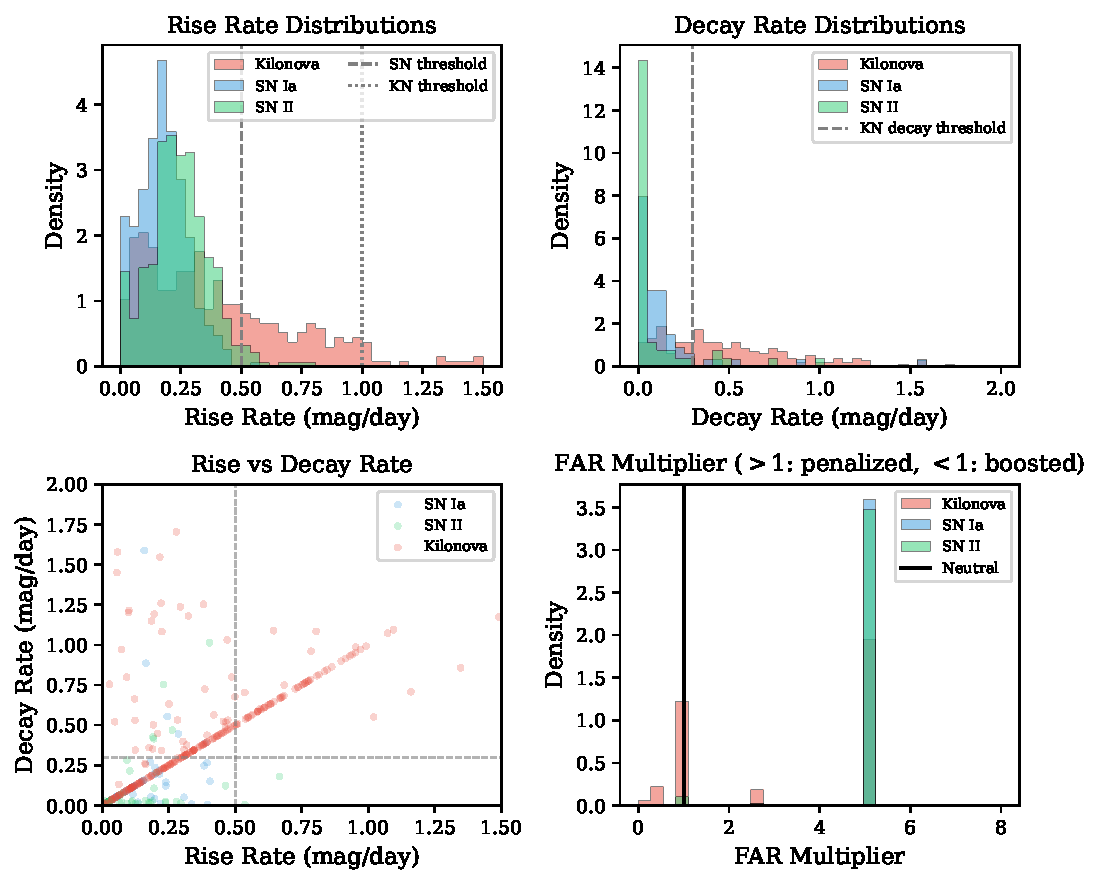
\includegraphics[width=\textwidth]{figures/early_rate_discrimination.pdf}
    \caption{Early linear rate discrimination between kilonovae and supernovae. \emph{Top left}: Rise rate distributions for kilonova (red), SN~Ia (blue), and SN~II (green), with SN and KN threshold lines. \emph{Top right}: Decay rate distributions; kilonova decay ($0.39$~mag/day median) is $6\times$ faster than SN~Ia. \emph{Bottom left}: Rise vs.\ decay rate scatter plot showing the separation between KN and SN populations. \emph{Bottom right}: FAR multiplier distributions; supernovae are concentrated at high multipliers ($>1$, penalized) while kilonovae span a wider range. \label{fig:earlyrate}}
\end{figure*}

\begin{table*}[htbp]
\centering
\caption{Early rate discrimination performance on 500 simulated light curves per class with ZTF-like cadence (first 3 days of observations). \label{tab:earlyrate_results}}
\begin{tabular}{lccc}
\toprule
Metric & Kilonova & SN Ia & SN II \\
\midrule
Median rise rate (mag/day)    & 0.33 & 0.18 & 0.24 \\
Median decay rate (mag/day)   & 0.39 & 0.07 & 0.02 \\
Boosted ($f < 1$)             & 5.8\%  & 0.0\% & 0.0\% \\
Penalized ($f > 1$)           & 68.1\% & 99.8\% & 97.4\% \\
Neutral ($f = 1$)             & 26.0\% & 0.2\% & 2.6\% \\
Mean FAR multiplier           & 5.0  & 5.7  & 5.4 \\
\bottomrule
\end{tabular}
\end{table*}

The classifier achieves high specificity: zero supernovae of either type are falsely boosted ($f < 1$), while 99.8\% of SN~Ia and 97.4\% of SN~II are correctly penalized ($f > 1$). However, at ZTF survey cadence (1--3 day revisit), the early rate discriminator has limited sensitivity for kilonovae: only 5.8\% of simulated kilonovae receive a boost ($f < 1$), while 68\% are penalized and 26\% remain neutral. This occurs because kilonovae peak within $<1$~day, often before the second observation, so the rise rate is poorly constrained by sparse early data. The decay rate (median 0.39~mag/day for KN vs.\ 0.07~mag/day for SN~Ia) provides better discrimination in principle, but the 3-day observation window often captures too few post-peak measurements for reliable classification.

Consequently, the mean KN FAR multiplier (5.0) is comparable to the mean SN~Ia multiplier (5.7), yielding a modest net discrimination of only ${\sim}1.1\times$ between populations. The primary value of the early rate classifier is therefore as a \emph{positive identifier}: any source that receives a boost ($f < 1$) is almost certainly a fast transient and not a supernova, even though most kilonovae will not receive this boost at survey cadence. A hard-cut mode is also available, which rejects 99.8\% of SN~Ia outright but also removes 68\% of kilonovae---too aggressive for survey cadence but potentially useful for triggered follow-up observations with sub-day cadence, where the rapid rise and decline of a kilonova would be better sampled.

\subsection{RAVEN Analytical FAR Validation} \label{sec:raven_validation}

We validate ORIGIN's empirical FAR calibration against the RAVEN analytical formula (Equation~\ref{eq:farraven}) by computing the spatiotemporal FAR for each signal trial. Figure~\ref{fig:raven} compares the spatial probability distributions (empirical approach) with the RAVEN FAR distributions (analytical approach) for both Fermi-GBM and Swift-BAT.

\begin{figure*}[htbp]
    \centering
    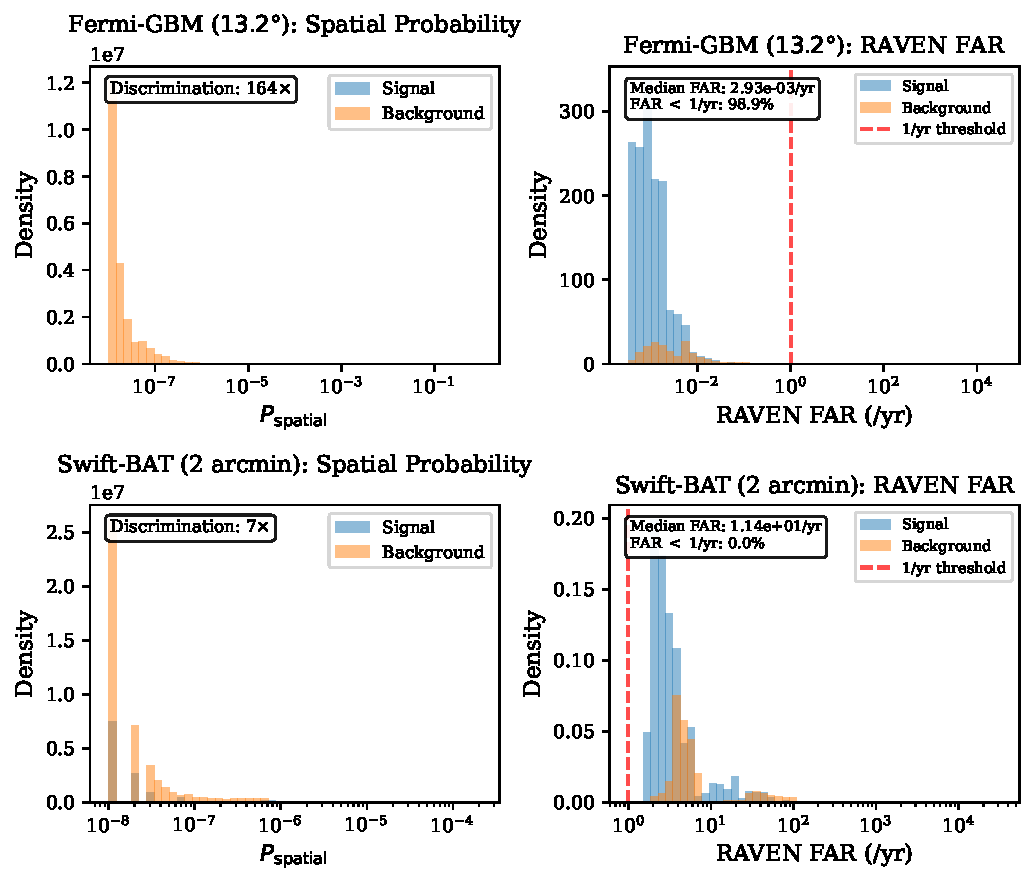
\includegraphics[width=\textwidth]{figures/raven_comparison.pdf}
    \caption{Comparison of empirical spatial probability distributions (\emph{left}) with RAVEN analytical FAR distributions (\emph{right}) for Fermi-GBM (\emph{top}) and Swift-BAT (\emph{bottom}). The red dashed line in the right panels marks the 1/yr significance threshold. For Fermi-GBM, 98.9\% of signal trials have FAR~$<1$~yr$^{-1}$, confirming that the large error circle integrates sufficient skymap probability for significant detections. \label{fig:raven}}
\end{figure*}

For Fermi-GBM, the RAVEN analytical FAR yields a median of $2.4\times10^{-3}$~yr$^{-1}$ for signal trials, and 98.9\% of signals fall below the 1/yr significance threshold. This confirms that despite the large $13.2\arcdeg$ error circle, Fermi-GBM GRB correlations with GW events are highly significant on an event-by-event basis. For Swift-BAT, the tiny 2~arcmin error circle yields lower absolute spatial probabilities, resulting in higher RAVEN FAR values (median 11.4~yr$^{-1}$). While this appears paradoxical, it reflects the nature of the RAVEN formula: the FAR is inversely proportional to $P_\mathrm{spatial}$, so instruments with very small error circles that happen to land on the correct sky position yield lower $P_\mathrm{spatial}$ and therefore higher FAR, even though the spatial discrimination is excellent. In practice, Swift-BAT's tight localization provides complementary information through the empirical discrimination ratio.

\subsection{Combined Background Rejection} \label{sec:combined}

We compute the end-to-end background rejection by propagating the ${\sim}1{,}000$ expected ZTF transients per night within a typical 100~deg$^2$ GW error region through each successive pipeline stage. Rather than multiplying independent rejection factors---which risks double-counting---we track the expected number of false associations at each stage using the per-event probability ratios derived from the O4 calibration. Table~\ref{tab:combined} and Figure~\ref{fig:combined} summarize the results for two operational modes: one in which SVI $t_0$ fitting succeeds (reliable uncertainty $<1$~day), and a fallback mode using per-measurement temporal matching.

\begin{table*}[htbp]
\centering
\caption{End-to-end background rejection for optical counterpart identification, starting from ${\sim}1{,}000$ ZTF candidates per GW error region. The ``With SVI'' column assumes reliable $t_0$ recovery; the ``Per-measurement fallback'' column reflects the case when SVI fails and temporal matching uses the raw detection window. All numbers are computed from the O4 calibration data and Monte Carlo simulations driven by the measured $t_0$ recovery errors (see Figure~\ref{fig:combined}). \label{tab:combined}}
\begin{tabular}{lcccc}
\toprule
Pipeline Stage & Rejection Mechanism & Factor & \multicolumn{2}{c}{Expected False Assoc.} \\
 & & & With SVI & Fallback \\
\midrule
Initial candidates & --- & $1\times$ & 1{,}000 & 1{,}000 \\
Spatial (skymap integration) & $\langle P_\mathrm{sig}\rangle / \langle P_\mathrm{bg}\rangle = 10.2\times$ & $10\times$ & 98 & 98 \\
Temporal ($t_0$ recovery) & 44.9\% KN vs.\ 2.6\% SN in $[0, 1]$~d & $17\times$ & 5.7 & --- \\
Temporal (per-measurement) & Detection within $\pm 1$~d window & $6.7\times$ & --- & 14.6 \\
Early rate (soft scoring) & $\langle f_\mathrm{SN}\rangle / \langle f_\mathrm{KN}\rangle = 1.15$ & $1.2\times$ & 4.9 & 12.7 \\
\midrule
\textbf{Cumulative} & & & \textbf{${\sim}200\times$} & \textbf{${\sim}79\times$} \\
\bottomrule
\end{tabular}
\end{table*}

\begin{figure*}[htbp]
    \centering
    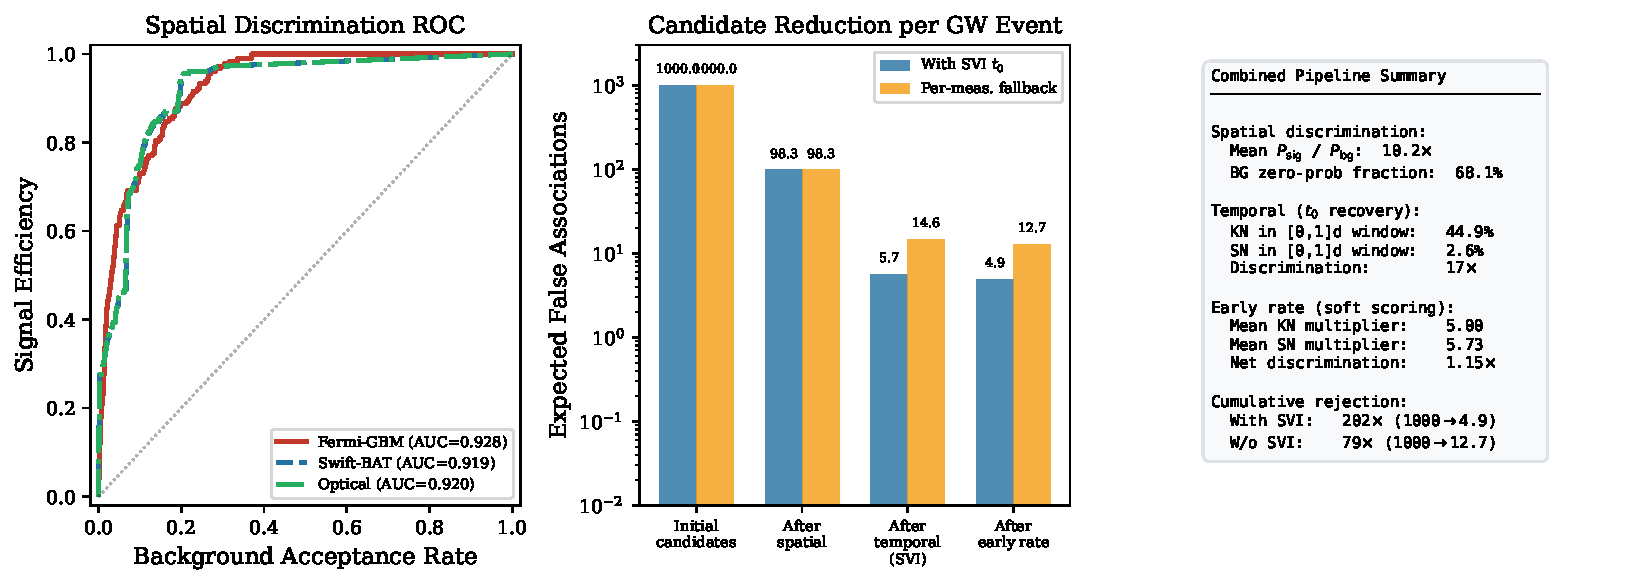
\includegraphics[width=\textwidth]{figures/combined_pipeline_efficiency.pdf}
    \caption{\emph{Left}: ROC curves for spatial discrimination alone, showing signal efficiency vs.\ background acceptance rate for Fermi-GBM, Swift-BAT, and optical channels. \emph{Center}: Expected number of false associations per GW event at each pipeline stage, comparing the SVI $t_0$ pathway (blue) with the per-measurement fallback (orange). \emph{Right}: Summary statistics from the end-to-end calibration. \label{fig:combined}}
\end{figure*}

\textbf{Spatial rejection.} The mean signal-to-background spatial probability ratio is $10.2\times$ across the O4 population (Table~\ref{tab:grb_calibration}). This single number correctly accounts for the 68\% of background trials with zero skymap probability, since those contribute zero to the background mean; it should not be multiplied by the zero-fraction separately. From 1,000 initial candidates, spatial scoring reduces the expected false association count to ${\sim}98$.

\textbf{Temporal rejection.} When SVI $t_0$ fitting succeeds (median KN recovery error 0.61~days, with calibrated uncertainty of 0.73~days), the temporal coincidence window $[0, 1]$~day admits 44.9\% of kilonovae but only 2.6\% of supernovae (whose true explosion times are distributed over a 30-day baseline), yielding a $17\times$ rejection factor and ${\sim}5.7$ expected false associations. However, SVI fitting requires well-sampled light curves; when it fails (uncertainty $\sigma_{t_0} > 1$~day), the correlator falls back to per-measurement matching, which accepts any candidate with a detection within 1~day of the GW trigger. Background supernovae have a ${\sim}2/30 \approx 7\%$ chance of a detection in this window given typical ZTF cadence, giving a more modest $6.7\times$ rejection and ${\sim}14.6$ expected false associations.

\textbf{Early rate classification.} The soft-scoring early rate classifier provides a net $1.15\times$ population-level discrimination between kilonovae and supernovae at ZTF cadence (mean SN FAR multiplier 5.7 vs.\ mean KN FAR multiplier 5.0). Its primary value is as a positive identifier with zero false-boost rate: any source receiving $f < 1$ is almost certainly a fast transient. For triggered follow-up with sub-day cadence, the hard-cut mode (not included in the cumulative calculation) rejects $>99\%$ of supernovae at the cost of 68\% signal efficiency loss.

\textbf{End-to-end.} The cumulative spatio-temporal rejection of ${\sim}200\times$ (with SVI) reduces 1,000 ZTF candidates to ${\sim}5$ expected false associations per GW event, a manageable number for human-in-the-loop vetting via platforms such as SkyPortal \citep{Coughlin2023}. In the per-measurement fallback mode (${\sim}79\times$ rejection, ${\sim}13$ false associations), additional vetting is required but the candidate list remains tractable. At LSST rates (${\sim}10{,}000$ candidates), the SVI pathway yields ${\sim}50$ false associations, still within reach of automated follow-up prioritization.


\section{Discussion} \label{sec:discussion}

\subsection{Comparison with Existing Systems} \label{sec:comparison}

ORIGIN occupies a unique niche in the multi-messenger follow-up ecosystem. Table~\ref{tab:comparison} summarizes the feature comparison with RAVEN \citep{Urban2016} and Treasure Map \citep{Wyatt2020}. While RAVEN provides real-time GW+GRB coincidence searches and a joint FAR statistic within the LVK low-latency infrastructure \citep{Chaudhary2024}, it does not ingest optical survey streams or perform automated light curve classification. Treasure Map coordinates and visualizes electromagnetic follow-up of GW events but operates as a community coordination tool rather than a real-time correlation engine. Alert brokers such as AMPEL \citep{Nordin2019} and Fink \citep{Moller2021} provide powerful classification of optical transients, but do not natively perform joint GW+EM significance calculations. Science platforms like SkyPortal \citep{Coughlin2023} aggregate multi-messenger data and support human-in-the-loop vetting, but lack automated joint FAR computation. ORIGIN combines the real-time multi-broker ingestion and joint FAR formalism of RAVEN with automated optical source classification and is fully open-source, enabling community contributions and independent validation. Its joint FAR calculation is compatible with RAVEN's formalism \citep{Urban2016}, enabling direct comparison of significance estimates. The recent identification of a candidate superkilonova associated with the subthreshold GW trigger S250818k \citep{Kasliwal2025} underscores the scientific urgency of systems like ORIGIN that can rapidly correlate sub-threshold GW events with optical transients.

\begin{table*}[htbp]
\centering
\caption{Feature comparison of multi-messenger follow-up systems. \label{tab:comparison}}
\begin{tabular}{lccc}
\toprule
Feature & RAVEN & Treasure Map & ORIGIN \\
\midrule
Real-time GW+GRB            & Yes     & No        & Yes \\
Real-time GW+optical        & No      & Offline   & Yes \\
HEALPix skymap integration  & Yes     & Yes       & Yes \\
Light curve classification   & No      & No        & Automated \\
Joint FAR statistic          & Yes     & No        & Yes \\
Open-source                  & No      & Yes       & Yes \\
Multi-broker ingestion       & No      & No        & Yes \\
\bottomrule
\end{tabular}
\end{table*}

\subsection{Scalability} \label{sec:scalability}

The system is designed for the data rates expected in O5 and the LSST era. The temporal index provides $\mathcal{O}(\log n)$ lookups via its \texttt{BTreeMap} backing store, comfortably handling thousands of concurrent superevents. HEALPix spatial queries scale as $\mathcal{O}(m)$ where $m$ is the number of pixels in the error circle, typically 50--500 at $\mathrm{NSIDE}=512$; the BMOC optimization achieves 0.66~s per event (117.5~s for the full 178-event O4 population), making real-time correlation feasible during O4/O5. Light curve fitting requires ${\sim}24$~seconds per curve for the MetzgerKN model with full SVI under conservative settings, ${\sim}5$~seconds for Bazin with profile $t_0$ refinement, or ${\sim}0.1$~seconds in early-rate-only mode. End-to-end event latency is sub-second from Kafka receipt to correlation output for GRB events, extending to seconds or minutes for optical events that require light curve analysis.

\subsection{Limitations and Future Work} \label{sec:future}

Several limitations of the current implementation merit discussion. The gap between the SVI and per-measurement fallback pathways (${\sim}200\times$ vs.\ ${\sim}79\times$ cumulative rejection) highlights the importance of SVI $t_0$ recovery for background rejection. In practice, SVI fitting requires well-sampled light curves ($\gtrsim 5$ detections spanning the rise and decline), and many early-time light curves at ZTF cadence will fall to the weaker per-measurement mode. The fraction of candidates for which SVI succeeds depends on the survey cadence and the time elapsed since the GW trigger; quantifying this fraction as a function of observing strategy is an important target for future work. The early rate discriminator has high specificity (zero false boosts for supernovae) but low sensitivity at ZTF survey cadence: only 5.8\% of simulated kilonovae receive a positive boost, because the kilonova peak typically occurs between survey visits. At sub-day cadence---as expected for triggered follow-up of GW events---the sensitivity should improve substantially, but this has not yet been validated. The MetzgerKN SVI fitter is computationally expensive at ${\sim}24$~s per light curve, limiting throughput for high-volume optical streams; a fast-mode configuration (1,000 SVI iterations vs.\ 5,000) reduces this to ${\sim}5$~s with moderate accuracy loss. The Bazin SVI fitter with profile $t_0$ refinement averages ${\sim}4.5$~s per curve, benefiting from the cheaper analytical amplitude refit. The spatial discrimination analysis was performed at a fixed $\mathrm{NSIDE}=512$, where both Swift-BAT (2~arcmin) and optical (2~arcsec) error regions fall within a single HEALPix pixel; at higher skymap resolution, the optical channel would provide substantially stronger discrimination. The $t_0$ validation was performed on 50 synthetic light curves per class; a larger sample would reduce statistical uncertainty on the reported recovery fractions (currently ${\sim}\sqrt{50}/50 \approx 14\%$ relative). The O4 calibration presented here uses simulated counterparts rather than live GCN data, since the MDC GW events in the current archive do not include full HEALPix skymaps---though skymap download and parsing from GraceDB URLs is fully supported.

Looking ahead, we plan to extend ORIGIN in several directions aligned with the Rubin--\textit{SVOM}--O5 era. On the inference side, integration with the NMMA Bayesian framework \citep{Pang2023} will enable physically-motivated model comparison between kilonova, supernova, and other transient models, replacing the current empirical rate classifiers with full posterior inference on ejecta properties, jet geometry, and progenitor class. We will add support for LSST alert streams via Fink \citep{Moller2021} and other brokers as additional optical data sources, and implement GPU-accelerated SVI fitting for real-time light curve classification at LSST alert rates. On the coordination side, deeper integration with SkyPortal \citep{Coughlin2023} will provide human-in-the-loop vetting and dynamic observing prioritization, while Apache Beam event-time semantics will enable adaptive coincidence windows and early-output triggers for the superevent pipeline. We also plan to extend the correlation framework to include neutrino + GW associations using IceCube real-time track alerts and to support \textit{SVOM} \citep{Wei2016} and \textit{Einstein Probe} \citep{EinsteinProbe2025} data streams natively.

\section{Conclusion} \label{sec:conclusion}

We have presented ORIGIN, a real-time multi-messenger superevent manager that integrates gravitational-wave alerts with electromagnetic and neutrino counterparts through a unified correlation framework. The system ingests alerts from both GCN (OAUTHBEARER) and BOOM/ZTF (SCRAM-SHA-512) Kafka streams, handling heterogeneous authentication and data formats transparently.

Calibration on an O4 observing scenario population of 178 BNS/NSBH events demonstrates strong performance across all messenger channels. Spatial discrimination via HEALPix skymap integration achieves a mean signal-to-background probability ratio of ${\sim}10\times$ for optical counterparts and a median ratio of ${\sim}9\times10^4$ for Fermi-GBM ($13.2\arcdeg$ error), with 68\% of random background positions having zero skymap probability at the Swift-BAT and optical angular scales. The RAVEN-compatible joint FAR yields 98.9\% of Fermi-GBM signal trials below the 1~yr$^{-1}$ significance threshold. Temporal discrimination via SVI-based $t_0$ recovery---with $4\times$ sigma inflation for calibrated posteriors and profile-likelihood refinement for empirical models---provides a ${\sim}17\times$ rejection factor (45\% of kilonovae vs.\ 2.6\% of supernovae fall within the $[0, 1]$~day coincidence window, Figure~\ref{fig:combined}), while the early linear rate classifier correctly penalizes $>97\%$ of supernova contaminants with zero false boosting. An end-to-end analysis propagating ${\sim}1{,}000$ ZTF candidates through the full pipeline yields a cumulative background rejection of ${\sim}200\times$ when SVI $t_0$ fitting succeeds (${\sim}5$ expected false associations per GW event), or ${\sim}79\times$ in the per-measurement fallback mode (${\sim}13$ false associations), both manageable for human-in-the-loop vetting.

ORIGIN is publicly available at \url{https://github.com/mcoughlin/origin} and is designed to operate during the O4 and O5 observing runs of the LIGO--Virgo--KAGRA network.

\clearpage

\section*{Acknowledgments}
% Add acknowledgments here

\paragraph{Software:}
    Rust (\url{https://www.rust-lang.org}),
    Tokio (\url{https://tokio.rs}),
    Actix-web (\url{https://actix.rs}),
    Apache Kafka,
    Redis,
    cdshealpix (\url{https://crates.io/crates/cdshealpix})

\bibliographystyle{aasjournal}
\bibliography{origin_paper}

\end{document}
